\documentclass{article}
\usepackage{float}
\usepackage{amsmath,amssymb,amsthm}
\usepackage{graphicx}
\usepackage{hyperref}
\setlength{\oddsidemargin}{0.25 in}
\setlength{\evensidemargin}{-0.25 in}
\setlength{\topmargin}{-0.6 in}
\setlength{\textwidth}{6.5 in}
\setlength{\textheight}{8.5 in}
\setlength{\headsep}{0.75 in}
\setlength{\parindent}{0 in}
\setlength{\parskip}{0.1 in}

\newtheorem{theorem}{Theorem}
\newtheorem{corollary}{Corollary}
\newtheorem{proposition}{Proposition}
\newtheorem*{remark}{Remark}
\theoremstyle{definition}
\newtheorem{example}{Example}
\newtheorem{definition}{Definition}

\newcommand{\lecture}[4]{
   \pagestyle{myheadings}
   \thispagestyle{plain}
   \newpage
%   \setcounter{lecnum}{#1}
   \setcounter{page}{1}
   \noindent
   \begin{center}
   \framebox{
      \vbox{\vspace{2mm}
    \hbox to 6.58in { {\bf CSC~565: Graph Theory
                        \hfill North Carolina State University} }
    \hbox to 6.58in { {\bf Fall 2019
                        \hfill Computer Science} }
       \vspace{4mm}
       \hbox to 6.28in { {\Large \hfill Lecture #1: #2  \hfill} }
       \vspace{2mm}
       \hbox to 6.28in { {\it Lecturer: {\it Don Sheehy {\tt <drsheehy@ncsu.edu>}} \hfill Scribe: #4} }
      \vspace{2mm}}
   }
   \end{center}
   \markboth{Lecture #1: #2}{Lecture #1: #2}
   \vspace*{4mm}
}


\begin{document}

  \title{Lecture 21}
  \author{Scribed by: Ellis Ackerman and Roshani Narasimhan}
  \date{November 4, 2019}
  \maketitle
  \noindent \textbf{Play with planarity}
  Game called "Planarity" gives a scrambled planar graph, where you can move around the vertices to find an embedding of the graph (no crossings). \href{http://planarity.net}{http://planarity.net}
  
  \noindent \textbf{Tutte's Algorithm}
  
  \textit{Goal} Find a linear embedding of a planar graph.
  \noindent \textit{Prerequisites for Tutte's algorithm} We need the graph to be a 3-connected graph.
  \newline \noindent \textit{Why do we need a 3-connected graph for Tutte's Algorithm?} Let $G$ be a 3-connected and planar graph. We need to fix an outer-face and we can do this since the faces are the non-separating induced cycles of $G$. Thus we know the edges that will bound a face.
  In the original version of Tutte's Algorithm, there are two steps:
  \begin{itemize}
      \item Fix the outer face - the vertices are placed equally-spaced on the circumference of a circle.
      \item Each of the other vertices is placed in the interior, at the centroid of its neighbors. 
  \end{itemize} 
  \noindent \textit{Does Tutte's Algorithm terminate eventually?}
  Say we put a vertex in the interior, at the centroid of its neighbours, then this system will have a new centroid and so on.
  This is equivalent to letting a spring system enter an equilibrium state, assuming all the springs have the same spring constant and the forces exerted by the neighbors, on the vertex at the centroid cancel out each other. Thus adding new vertices inside would at some point of time bring the system in equilibrium, thus a solution exists and the algorithm converges.  
  The condition stated above imposes two linear constraints for each vertex in the interior, as is evident from the Hooke's law - one in the $x$ direction and one in the $y$ direction.
  
  \noindent \textit{Solutions obtained from the algorithm}
  We formalize this notion using block-matrices. $$LP = \bmat{F\\0},$$ where $L$ is the Laplacian of $G$ and $P$ are the positions of all vertices. $F$ are the forces on the vertices of the outer face, and $0$ corresponds to the fact that the center of the system, which consists of internal vertices, is at equilibrium. This matrix system tells us that, $$\bmat{L_1 & B \\ B^T & L_2}\bmat{P_{\text{out}}\\P_{\text{in}}} = \bmat{F\\0}.$$ Here $L_1$ and $L_2$ are the parts of the Laplacian which correspond to the Laplacians of the outer and inner faces, respectively. By matrix-block multiplication, we have, $$L_2P_{\text{in}} = -B^TP_{\text{out}}.$$ By inverting $L_2$, we would be able to solve this system for $P_{\text{in}}$, which would result in the locations of inner vertices, based on the positions of the outer vertices.
  
  \noindent \textit{How many solutions are possible?}
  Maxwell observed that sometimes, there is not just one 'reciprocal diagram' but a family of 'reciprocal diagrams' (which obtained from the solution of the rows/columns of the matrix which are not linearly dependent on each other).
  If $L_2$ is not invertible, there could be many solutions to this system. Recall that by the \textit{Matrix-Tree Theorem} (which states that the determinant of the Laplacian with first row and first column removed is the number of spanning trees of G), $L_2$ is indeed invertible (has a positive determinant). Thus, we can solve for for the locations of the interior vertices, $$P_{\text{in}} = -L_2^{-1}B^T P_{\text{out}}.$$
  
  \textit{What could go wrong if G was not 3-connected?} Let us consider the example of a $K_3$ subgraph in $G$. If we want to add the third vertex, then it should be placed at the then the centroid for the two vertices. The centroid would lie on the edge connecting the two vertices, thus adding the third vertex would result in overlapping of edges. The figure below illustrates this notion.
  
  \medskip \noindent 
      \begin{figure}[H]
    \centering
    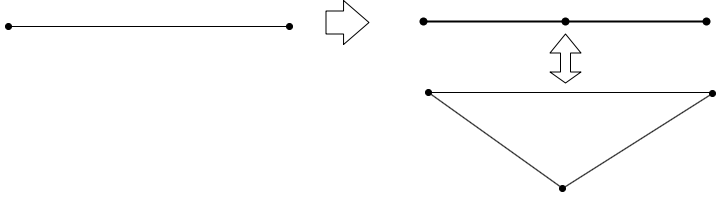
\includegraphics[scale=0.5]{Images/k3_centroid.png}
    \caption{Adding a vertex to the interior of two existing vertices results in a line with overlapping edges instead of forming a triangle.}
    \label{fig:my_label}
    \end{figure}
  
    \medskip \noindent So how do we prove that this algorithm is correct and is an embedding of the graph, and not just a drawing? If we return to thinking of the edges as springs in equilibrium, then we are essentially thinking of a net as we stretch the outer-face of the graph. If we try to pull away of crossings, we create monotone paths (edges increasing in one direction) in the drawing. We note that faces must be convex. A polygon is not convex if it has a \textbf{reflex vertex} or a \textbf{winding}. In both these cases, we can find a line in the plane that separates the four vertices into two sets, thereby creating monotone paths between the interleaved vertices. This indeed creates a $K_4$ topological minor and we know that a graph containing $K_4$ topological minor is not planar.
  
    % NEED TO RE-POSITION THE FIGURES
   % image for reflex vertex -- showing monotone paths
    \begin{figure}[H]
    \centering
    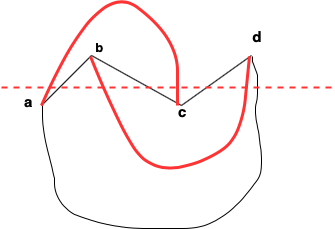
\includegraphics[scale=0.5]{Images/monotone_paths_in_reflex_vertices.png}
    \caption{Note the monotone paths marked in red from a to c and b to d, when the graph contains reflex vertices. The graph shown above is not planar.}
    \label{fig:my_label}
    \end{figure}
   
   % image showing winding
    \begin{figure}[H]
    \centering
    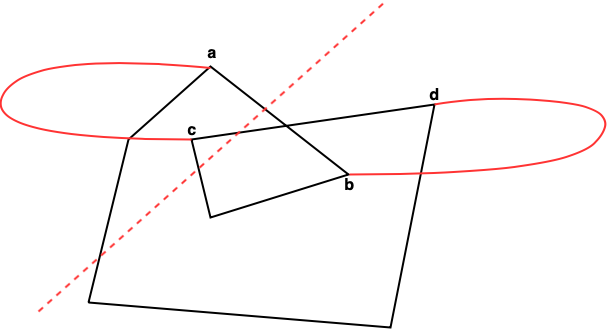
\includegraphics[scale=0.5]{Images/winding_polygon.png}
    \caption{Note the monotone paths marked in red from a to c and b to d, when the graph contains a winding. The graph shown above is not planar.}
    \label{fig:my_label}
    \end{figure}

    \medskip \noindent The goal now is to show that as we glue various faces (which we have asserted to be convex polygons) of $G$ together, they do not overlap. We do this by showing that locally, there are no crossings. 
    
    \medskip \noindent \textbf{Definition:} Ply is the number of polygons at any point. This is a function on the plane. For each point in the plane, it returns the number of polygons "stacked" at that point. 
    \medskip \noindent Thus, our goal becomes checking at the alleged embedding by Tutte's Algorithm yields a drawing in which the ply is one inside the drawing and zero out outside of it. This will be good to show that there are no crossings.
    
    \medskip \noindent We must check the following:
    \begin{itemize}
        \item For every edge in $G$, \textbf{faces are on opposite sides of the shared edge}. If the faces are on the same side of an edge, it means there is an overlap of faces. This implies that the ply is greater than 1. We can think of this as a sheet of paper being folded into two. The crease signifies the shared edge and surfaces of the paper denote the ply (which is equal to 2).
        
        % ply with edges on the same side
        \begin{figure}[H]
        \centering
        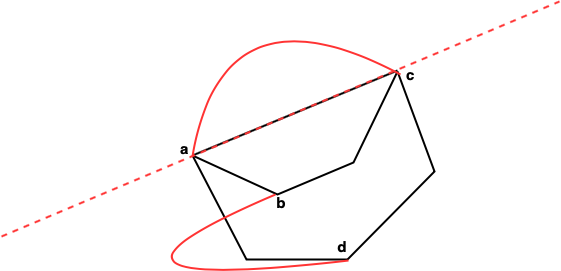
\includegraphics[scale=0.5]{Images/shared_edge_ply.png}
        \caption{This figure shows that though there are no explicit crossings in the drawing of the graph, there is a shared edge, which makes the ply equal to two in certain portion of the drawing. Note the monotone paths marked in red from a to c and b to d, when the graph contains a winding. Tutte's algorithm would not yield such a drawing.}
        \label{fig:my_label}
        \end{figure}
    
    
        \item We must also check that there is \textbf{no winding around a vertex}, when we are gluing the polygons together. We ensure this by checking that the sum of the angles of the edges coming out of the vertex are less than $2 \pi$. If there is a winding around a particular vertex, it means that we circle about more than once, which is possible only when there is a crossing among one or more edges. This means that we can find monotone paths between two points on different winding (which will lead to a $K_4$ topological minor, which has 4 vertices on same face). Thus the existence of monotone paths imply existence of sub-graphs that cannot exist in a planar graph.
        
        % winding around a vertex
        \begin{figure}[H]
        \centering
        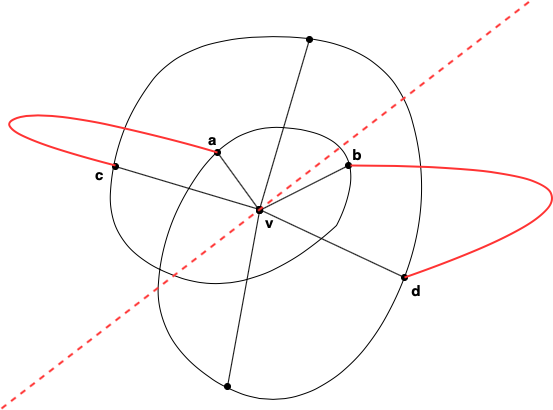
\includegraphics[scale=0.5]{Images/winding_around_a_vertex.png}
        \caption{Around the vertex v, due to the winding we can find monotone paths between a and c ; b and d. Ply within the inner winding is 2. }
        \label{fig:my_label}
        \end{figure}
    \end{itemize} 
    

    
    \medskip \noindent \textbf {Locally "good" to globally "good"}
    \textit{If G satisfies conditions locally, does it ensure that G has a planar embedding?}

     %figure of a cube with crossings
        \begin{figure}[H]
        \centering
        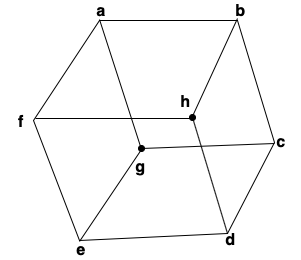
\includegraphics[scale=0.5]{Images/cube.png}
        \caption{Drawing for a cube which does not comply with Tutte's algorithm. This drawing has the inner vertices g and h placed at the centroid of its neighbouring vertices. However the outer hexagon formed by a,b,c,d,e and f does not form a face.}
        \label{fig:my_label}
        \end{figure}

    \medskip \noindent Let us consider the drawing of the cube provided above. We note that:
    \begin{itemize}
        \item The internal vertices are placed at the centroid of its neighbours. (The forces of exerted by the outer vertices are balanced at the inner vertices). 
        \item At the internal vertices, there is no winding, which means that the angles made by the edges at these vertices are equal to $2 \pi$.
        \item Each edge has faces to the opposite sides. 
        \item Faces look to be convex, however the outer face is not actually a face of the cube! The outer hexagon is not a non-induced separating cycle. Recall that it is important that the outer-face of the embedding of the graph, must be a non-separating induced cycle (implied by the fact that the graph is 3-connected). 
        \item We observe crossings at edges as well. 
        \item Ply is two everywhere inside the embedding. 
    \end{itemize}
    Thus even though the local conditions for the vertices and the edges are satisfied, we note that the above drawing of a cube is not a planar embedding.
  %[ENTER FIGURE explain the ply and how it is an incorrect implementation] Ellis, please let me know which figure this would be! I am pretty sure I was thinking this one would be the cube with the hexagon outer face so we are good!%
  
     
    \medskip \noindent Interesting facts about ply:
    \begin{itemize}
        \item For a planar graph, ply does not change at the edges - as faces are on the opposite sides of the edge.
        \item Ply will be constant at a vertex, as the number of polygons which meet at the vertex must be constant.
        \item For a planar graph, the ply in the inner faces of the graph is 1 and the ply outside of the outer face is 0.
    \end{itemize}
    
    % x to y figure in planar graph
    \begin{figure}[H]
    \centering
    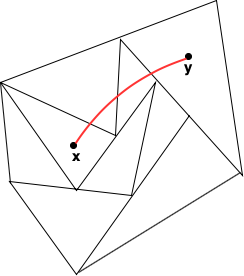
\includegraphics[scale=0.5]{Images/change_of_ply_from_x_to_y.png}
    \caption{Tracking change in the ply at two points x and y within the graph.}
    \label{fig:my_label}
    \end{figure}
    \medskip \noindent We now consider the ply and the drawing of the graph above. Let us assume that for two points, $x$ and $y$ in the graph, $\text{ply}(x) \neq \text{ply}(y)$. If something is not true globally, then it must be not true somewhere locally. Thus, if we "walk" from $x$ to $y$, then at some point the ply must change, i.e. a boundary is crossed. But we have shown that locally the embedding is well-behaved. The ply is constant on the interior on edges and vertices. Thus the ply can only change when the outer-face is crossed. 
    
    \medskip \noindent \textbf{Lingering Issues and Problem Variations}
  
     \medskip \noindent \textit{Mean Graphs}
  \newline \noindent Consider the graph $K_3 \times P_{n/3}$. The center section gets smaller and smaller. These sort of situations can be hard for computers to represent and we can run into numerical precision errors. 
  % figure of K3 * Pn/3
    \begin{figure}[H]
    \centering
    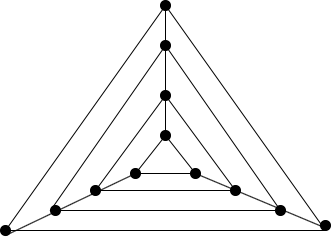
\includegraphics[scale=0.5]{Images/clique_cross_path.png}
    \caption{$K_3 \times P_{n/3}$ as a computationally difficult problem.}
    \label{fig:my_label}
    \end{figure}  
  
    \medskip \noindent \textit{Low-Precision Embdeddings}
  \newline \noindent Can we embed a graph into the plane such that the vertices are on grid points. The original embedding problem let us place vertices at any point in the real plane, but this variation now constricts us to the integers, changing the allowed precision. Many problems become harder under this restriction, including graph embeddings. %[ENTER FIGURE] Ellis, please let me know which figure this would be%
  
    \medskip \noindent \textit{Spectral Graph Embedding}
  \newline \noindent Instead of solving the linear system, we consider the eigenvalues of the Laplacian for each direction, $$Lx=\lambda x \text{ and } Ly=\lambda y.$$
  We are looking for the force vectors directed towards or away from the origin. While this method does not give us force equilibrium as Tutte's Algorithm does, it does give us an organized way to embed the graph. This method leads to the notion of "scaling". Note that $L$ has $n-1$ eigenvectors and it is not always clear which is "best." This method was first discussed in applications of computational chemistry.

\end{document}
